% !TeX root = ../../../main.tex

\subsection{Corpora, Reference Annotations, and Model Configurations}\label{ch05:apd:corpora-configurations}

Table~\ref{ch06:tab:dataset-summary} summarizes the evaluation populations and their reference annotations.

Figures~\ref{ch05:fig:record_schema} and~\ref{ch05:fig:demo} show the PMOA-TTS record schema and cohort demographics.

% !TeX root = ../../../../main.tex
\subsubsection{Annotated PMOA Subsets}
\label{ch06:apd:subset_ids}

The \texttt{sepsis-40} subset contains 40 PMOA case reports with manual clinician annotations, yielding $3,229$ reference clinical events.
The \texttt{sepsis-10} subset is a 10-report subset (801 reference events) of \texttt{sepsis-40} used for clinician annotation quality review, hallucination audit, multi-pass self-consistency, and sepsis onset analysis.


% !TeX root = ../../../../main.tex
\begin{table}[htbp]
\caption{
PMCID composition of the annotated PMOA subsets for \texttt{sepsis-40}.\\
A checkmark indicates membership in \texttt{sepsis-10}.
}\ChSixFloatLabel{ch06:tab:subset_pmcs}
\ChSixTableBodyStart
\begin{ChSixFloatBody}

\centering


\begin{tabular}{lc@{\hspace{3em}}lc}
\toprule
PMCID & \texttt{sepsis-10} & PMCID & \texttt{sepsis-10} \\
\midrule
PMC10037274 &  & PMC10493687 &  \\
PMC3075162  & \checkmark & PMC4421677  &  \\
PMC4929359  &  & PMC5862012  &  \\
PMC6345085  &  & PMC7331532  &  \\
PMC8546416  &  & PMC9355071  & \checkmark \\
PMC10370906 & \checkmark & PMC10556716 & \checkmark \\
PMC3130983  &  & PMC4573216  &  \\
PMC5142474  &  & PMC6059163  &  \\
PMC6441647  &  & PMC7451141  &  \\
PMC8855197  &  & PMC9393191  &  \\
PMC10406025 &  & PMC10629858 & \checkmark \\
PMC3325348  &  & PMC4778217  & \checkmark \\
PMC5721301  &  & PMC6231299  &  \\
PMC6910033  &  & PMC7576661  & \checkmark \\
PMC9136437  & \checkmark & PMC9552858  & \checkmark \\
PMC10480000 &  & PMC2698425  &  \\
PMC4120057  &  & PMC4898175  &  \\
PMC5747955  &  & PMC6238558  & \checkmark \\
PMC7093739  &  & PMC8298783  &  \\
PMC9260376  &  & PMC9647393  &  \\
\bottomrule
\end{tabular}

\end{ChSixFloatBody}
\end{table}


\FloatBarrier

% !TeX root = ../../../main.tex
\begin{figure}[htbp]
\begin{ChFiveFloatBody}

\centering

\begin{minipage}[t]{1\textwidth}
\centering
\footnotesize
\begin{adjustbox}{max width=\linewidth}\begin{tabular}{@{} l l >{\raggedright\arraybackslash}p{4cm} @{}}
\toprule
\textbf{Field} & \textbf{Type} & \textbf{Description} \\
\midrule
\texttt{pmc\_id} & str &
Folder-level ID (PMC000xxxxxx--PMC011xxxxxx). \\

\texttt{case\_report\_id} & str &
Filename of the case (e.g., PMC6417290). \\

\texttt{textual\_timeseries} & List[Dict] &
Sequence of \{"event": str, "time": int\}. \\

\texttt{demographics} & Dict &
\{"age": str/"Not Specified", "sex": str, "ethnicity": str\}. \\

\texttt{diagnoses} & List[str] &
List of diagnosis terms extracted per case. \\

\bottomrule
\end{tabular}\end{adjustbox}
\end{minipage}
\hfill

\begin{minipage}[t]{\linewidth}
\centering
\begin{tcolorbox}[
  colback=gray!5,
  colframe=gray!70,
  title=Example JSON entry,
  boxrule=1pt,
  enhanced,
  %breakable,
  fontupper=\footnotesize
]
\begin{verbatim}
"pmc_id": "PMC006xxxxxx",
"case_report_id": "PMC6417290",

"textual_timeseries": [
  {"event": "56 years old", "time": 0},
  {"event": "male", "time": 0},
  {"event": "HIV-positive", "time": 0},
  {"event": "admitted to the hospital", "time": 0},
  {"event": "knee arthralgia", "time": 0},
  ...
  {"event": "postural headache", "time": 48},
  {"event": "neurological examination", "time": 120},
  {"event": "persistence of headache", "time": 144},
  {"event": "brain computed tomography scan",
   "time": 144},
  ...
  {"event": "symptom free", "time": 4320},
  {"event": "CT scan", "time": 4320},
  {"event": "no brain shift", "time": 4320}
],
"diagnoses": [
  "HIV",
  "Knee arthralgia",
  "Subdural hematoma",
  "Postdural puncture headache (PDPH)"
],
"demographics": {
  "age": 56,
  "sex": "Male",
  "ethnicity": "Not Specified"
}
\end{verbatim}
\end{tcolorbox}
\end{minipage}





\end{ChFiveFloatBody}
\caption{\textbf{top:} PMOA-TTS record schema. \textbf{bottom:} compact example matching the schema above (drawn from our HuggingFace repository (formatted for readability).}\ChFiveFloatLabel{ch05:fig:record_schema}
\end{figure}

% !TeX root = ../../../main.tex
\begin{figure}[htbp]
\begin{ChFiveFloatBody}

  \centering
  \begin{minipage}[t]{0.49\linewidth}
    \centering
    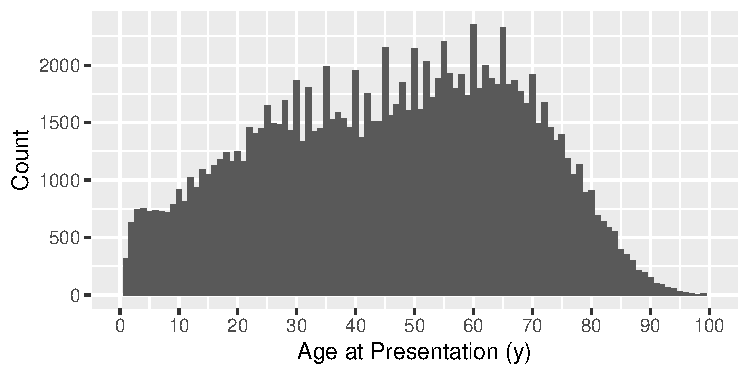
\includegraphics[width=\linewidth]{Appendices/appendix-ch05/images/Scientific_data/Plots_tables/125k_age.pdf}
  \end{minipage}\hfill
  \begin{minipage}[t]{0.49\linewidth}
    \centering
    \scriptsize
    \begin{tabular}{l r}
      \toprule
      \textbf{Characteristic} & \textbf{Percent (\%)}\\
      \midrule
      \multicolumn{2}{l}{\textbf{Sex}}\\
      \quad Male & 52\\
      \quad Female & 47\\
      \quad Not Specified & 1\\
      \midrule
      \multicolumn{2}{l}{\textbf{Ethnicity}}\\
      \quad White/Caucasian & 5\\
      \quad Asian & 3\\
      \quad African & 1\\
      \quad Other & 2\\
      \quad Not Specified & 89\\
      \bottomrule
    \end{tabular}
  \end{minipage}
  
  
  

\end{ChFiveFloatBody}
\caption{\ChFiveRebuttal{Age distribution and LLM-mapped/extracted demographic descriptors for 124{,}349 PMOA-TTS case reports.}}\ChFiveFloatLabel{ch05:fig:demo}
\end{figure}

\FloatBarrier

% !TeX root = ../../../main.tex
\subsubsection{UMLS Mapping for Diagnosis Standardization}
\label{ch05:apd:umls-mapping}

To standardize the diagnoses extracted by LLMs from the case reports, we mapped the free-text diagnoses to concepts in the Unified Medical Language System (UMLS). 
This process involved the following steps:

\begin{enumerate}
    \item \textbf{Initial Extraction}: For each case report, we prompted the LLM to extract diagnoses. 
    This yielded a list of free-text diagnoses for each case report.

    \item \textbf{Entity Linking}: We used ScispaCy's entity linker model 
    \texttt{(en\_core\_sci\_lg)} with the UMLS knowledge base to map each extracted diagnosis to corresponding UMLS Concept Unique Identifiers (CUIs). 
    \ChFiveRebuttal{Each complete extracted diagnosis string is now supplied directly to the UMLS candidate generator.}

    \item \textbf{Filtering and Disambiguation}: For each diagnosis, we:
    \begin{itemize}
        \item Retained only mappings with a confidence score above 0.85.
        \item \ChFiveRebuttal{When candidates are tied or near-tied, the selection procedure favors exact normalized canonical-name matches, recognized canonical suffixes, and concepts whose canonical name contains the complete diagnosis phrase.}
    \end{itemize}

    \item \textbf{Concept Normalization}: After mapping to CUIs, we:
    \begin{itemize}
        \item Retrieved the canonical names from UMLS Metathesaurus.
    \end{itemize}
\end{enumerate}


This mapping process allowed us to standardize the diverse expressions of diagnoses extracted by LLMs into a consistent terminology system, enabling more reliable frequency analysis and co-occurrence patterns. 
Across the full PMOA-TTS corpus, LLM-extracted diagnoses yielded
$N_{\text{raw}} = 63{,}715$ unique free-text diagnosis strings.
Of these, $N_{\text{mapped}} = 41{,}216$ ($64.7\%$) were successfully mapped to at least one
UMLS CUI with a confidence score $\ge 0.85$.
When weighted by frequency of occurrence, mappings at this threshold covered
$91.7\%$ of all diagnosis mentions, indicating that commonly occurring clinical
diagnoses were more likely to receive high-confidence mappings.
Mapping coverage decreased monotonically with increasing confidence threshold.
We therefore selected a threshold of 0.85 as a conservative operating point for
downstream normalization, providing broad coverage of frequently occurring diagnoses
while maintaining a high-confidence mapping criterion.


% !TeX root = ../../../main.tex
\subsubsection{Model and Inference Configuration}
\label{ch05:sec:supp-model-configuration}

Seven large language models were evaluated for textual time series annotation:
Llama 3.3 70B Instruct, DeepSeek-R1, DeepSeek-V3, GPT-5, O4-mini, O3,
and O1.
The exact checkpoint identifiers and Azure deployment names are
reported in Table~\ref{ch05:tab:model-identifiers}.
Llama 3.3 70B Instruct and
DeepSeek-R1 were also used to produce the full-corpus annotations.
Each model
was evaluated across five independent generation runs using the textual time
series prompt in Supplementary Section~\ref{ch05:apd:extraction-prompt}.


Table~\ref{ch05:tab:inference-settings} summarizes the recorded inference
configuration.
Llama 3.3 70B Instruct was run using Hugging Face Transformers
and PyTorch with bfloat16 weights and automatic device placement.
The Azure
OpenAI models were queried through the Chat Completions interface using API
version \texttt{2024-12-01-preview}.
Temperature, top-$p$, and generation seeds
were not explicitly specified for the Azure models.
In all API-based runs, the
complete extraction prompt and case-report text were submitted together as a
single user message, and responses were generated without streaming.


% !TeX root = ../../../main.tex
\begin{table}[htbp]
\caption{
Exact model identifiers and Azure OpenAI deployment names used for textual
time series annotation.
}\ChFiveFloatLabel{ch05:tab:model-identifiers}
\ChFiveTableBodyStart
\begin{ChFiveFloatBody}

\centering


\scriptsize
\setlength{\tabcolsep}{6pt}
\renewcommand{\arraystretch}{1.15}
\begin{tabular}{>{\raggedright\arraybackslash}p{0.31\linewidth} >{\raggedright\arraybackslash}p{0.61\linewidth}}
\toprule
\textbf{Model} &
\textbf{Checkpoint identifier or API deployment} \\
\midrule

Llama 3.3 70B Instruct &
\texttt{meta-llama/Llama-3.3-70B-Instruct} \\

DeepSeek-R1 &
\texttt{deepseek-ai/DeepSeek-R1-0528} \\

DeepSeek-V3 &
\texttt{deepseek-ai/DeepSeek-V3-0324} \\

GPT-5 &
Azure OpenAI deployment \texttt{gpt-5} \\

O4-mini &
Azure OpenAI deployment \texttt{o4-mini} \\

O3 &
Azure OpenAI deployment \texttt{o3} \\

O1 &
Azure OpenAI deployment \texttt{o1} \\

\bottomrule
\end{tabular}

\end{ChFiveFloatBody}
\end{table}



% !TeX root = ../../../main.tex
\begin{table}[htbp]
\caption{
Inference and generation settings used for textual time series annotation.
Parameters described as not explicitly set were not supplied in the
corresponding generation request.
}\ChFiveFloatLabel{ch05:tab:inference-settings}
\ChFiveTableBodyStart
\begin{ChFiveFloatBody}

\centering


\scriptsize
\setlength{\tabcolsep}{5pt}
\renewcommand{\arraystretch}{1.18}
\begin{tabular}{
    >{\raggedright\arraybackslash}p{0.18\textwidth}
    >{\raggedright\arraybackslash}p{0.28\textwidth}
    >{\raggedright\arraybackslash}p{0.47\textwidth}
}
\toprule
\textbf{Model or configuration} &
\textbf{Inference framework and precision} &
\textbf{Generation settings} \\
\midrule

Llama 3.3 70B Instruct
(full-corpus annotation) &
Hugging Face Transformers and PyTorch;
bfloat16;
automatic device placement &
128k-token model context;
batch size 1;
\texttt{max\_new\_tokens=8092};
\texttt{do\_sample=True};
\texttt{top\_k=1};
one returned sequence;
temperature and top-$p$ not explicitly set;
no explicit generation seed \\

Llama 3.3 70B Instruct
(technical validation) &
Hugging Face Transformers and PyTorch;
bfloat16;
automatic device placement &
128k-token model context;
batch size 1;
\texttt{max\_new\_tokens=8092};
\texttt{do\_sample=True};
\texttt{temperature=1};
\texttt{top\_k=1};
one returned sequence;
no explicit generation seed \\

DeepSeek-R1 &
DeepSeek-V3 architecture;
checkpoint configuration specifies bfloat16 with FP8 block quantization &
163{,}840-position context;
five independent generation runs using the production textual time series
prompt \\

DeepSeek-V3 &
DeepSeek-V3 architecture;
checkpoint configuration specifies bfloat16 with FP8 block quantization &
163{,}840-position context;
five independent generation runs using the production textual time series
prompt \\

GPT-5 &
Azure OpenAI Chat Completions;
provider-managed numerical precision &
API version \texttt{2024-12-01-preview};
\texttt{max\_completion\_tokens=16834};
\texttt{stream=False};
temperature, top-$p$, and API seed not explicitly set \\

O4-mini, O3, and O1 &
Azure OpenAI Chat Completions;
provider-managed numerical precision &
API version \texttt{2024-12-01-preview};
\texttt{max\_completion\_tokens=40000};
\texttt{stream=False};
temperature, top-$p$, and API seed not explicitly set \\

\bottomrule
\end{tabular}

\end{ChFiveFloatBody}
\end{table}


\subsubsection{Sepsis Reconstruction Study Configuration}

Table~\ref{ch06:tab:study-configuration} retains the sepsis study configuration, including the phenotype counts and reference models.

% !TeX root = ../../../../main.tex
\begin{table}[htbp]
\caption{Sepsis reconstruction study configuration. Bold cells indicate contributed labeling}\ChSixFloatLabel{ch06:tab:study-configuration}
\ChSixTableBodyStart
\begin{ChSixFloatBody}




\centering
\begin{adjustbox}{width=0.8\textwidth}
\begin{tabular}{|>{\raggedright\arraybackslash}p{3.5cm}|>{\raggedright\arraybackslash}p{3.5cm}|>{\raggedright\arraybackslash}p{3.5cm}|>{\raggedright\arraybackslash}p{3.5cm}|}
\hline
\textbf{Corpus}                  & \centering \textbf{i2m4}             & \centering \textbf{\texttt{sepsis-40}}& \textbf{\qquad \texttt{sepsis-100}}       \\
\hline
\textbf{N (unlabeled)}          & \multicolumn{1}{r|}{310;  331,794}             & \multicolumn{1}{r|}{2,139}                     & \multicolumn{1}{r|}{2,139}                      \\ \hline
\textbf{N (labeled)}            & \multicolumn{1}{r|}{20}                         & \multicolumn{1}{r|}{40}                       & \multicolumn{1}{r|}{100}                       \\ \hline
\textbf{Source}                 & i2b2; MIMIC IV           & PMOA       & PMOA       \\ \hline
\textbf{Note type}              & discharge summary        & case report              & case report               \\ \hline
\textbf{Labeler}                & \textbf{clinicians}               & \textbf{clinicians} (Gold)& \textbf{GPT-5} (Bronze)\\ \hline
\textbf{Phenotyper}             & \textbf{clinicians}      & \textbf{clinicians}      & \textbf{QwQ-32B-Preview}             \\ \hline
\textbf{Methods}                &                & GPT-5& GPT-5\\ 
                                & DeepSeek-R1& DeepSeek-R1& DeepSeek-R1\\ 
                                & L3.3 70B Instruct                  & L3.3 70B Instruct                & L3.3 70B Instruct                 \\ 
                                & L3.1 70B Instruct                 & L3.1 70B Instruct                & L3.1 70B Instruct   \\ 
                                & Mixtral 8x7B & Mixtral 8x7B                & Mixtral 8x7B                   \\ 
                                & \quad Instruct v0.1 & \quad Instruct v0.1                & \quad Instruct v0.1                   \\ 
                                & L3.1 8B Instruct             & L3.1 8B Instruct                & L3.1 8B Instruct                  \\ \hline
\parbox{3cm}{\textbf{Ablations}} & No role                  & No role                  & No role                   \\ 
Base: & No conjunction & No conjunction & No conjunction
                                \\ 
L3.3 70B Instruct                        & \quad instruction &  \quad instruction & \quad instruction \\
                                
                                & No few-shot prompting    & No few-shot prompting    & No few-shot prompting     \\ \hline
\textbf{Sensitivity analyses}   & With upper bound         & With upper bound         & With upper bound          \\ 
                                & With upper bound + 
                                                         & With upper bound +  
                                                                                      & With upper bound + \\
                                & \quad i2b2 event typing & \quad i2b2 event typing & \quad i2b2 event typing \\
                                                                                      \hline
\end{tabular}
\end{adjustbox}

\end{ChSixFloatBody}
\end{table}


\FloatBarrier
